\documentclass[a4paper,11pt, twocolumn]{article}
\usepackage[margin=0.8in]{geometry}
\usepackage{xcolor}
\usepackage{graphicx} %package to manage images
\graphicspath{ {./images/} }

\title{AS-4 Semiconductor Components}
\author{Revision sheet}
\date{}

\usepackage{fancyhdr}
\pagestyle{fancy}
\fancyhead{} % clear all header fields
\renewcommand{\headrulewidth}{0pt} % no line in header area
\fancyfoot{} % clear all footer fields
\renewcommand{\footrulewidth}{0.4pt}
\fancyfoot[C]{\thepage} % page number in centre of the page
\fancyfoot[R]{\footnotesize Thomas Boxall \\ Some images from WJEC E-Book} % right hand footer has author name on top line and images reference on bottom line
\fancyfoot[L]{\footnotesize AS-4 Semiconductor Components \\ Revision sheet} % left hand footer has title of document on top line and 'Revision Sheet' on bottom line


\begin{document}

\maketitle
\thispagestyle{fancy}

% CONTENTS OF THE REVISION SHEET HERE

\section{Diode}
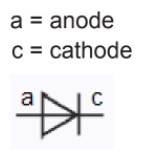
\includegraphics[width=0.15\textwidth]{diode.jpg}\\
The current can only flow in one direction, from the anode to the cathode. The anode is positive and the cathode is negative. 
\subsection{VI Characteristics}
Current will only flow when voltage across the diode is greater than 0.7V. \\
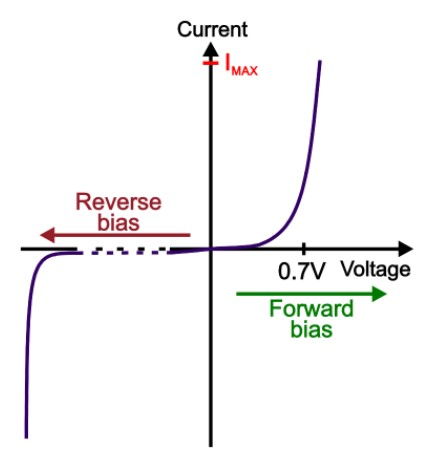
\includegraphics[width=0.45\textwidth]{diode vi characteristics.jpg}\\
As seen in the graph, if we apply enough voltage when in reverse bias, the diode will break (known as reverse breakdown) and current will flow. This is irreversible. 

\section{Bipolar Junction Transistor (BJT)}
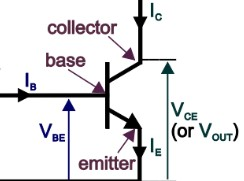
\includegraphics[width=0.3\textwidth]{bjt.jpg}\\
Transistors have three terminals - base, collector and emitter.
\subsection{What Do Transistors Do?}
Transistors are current amplifiers. A small current flowing form the base to the emitter, $I_B$, causes a much larger current to flow from the collector to the emitter. The equation $\displaystyle I_C = h_{FE} \times I_B$ links the collector and base currents. The $h_{FE}$ value is the current gain and is usually between 30 and 800; it will usually be in the question.
\subsubsection{Voltage in Transistors}
Transistors have a $0.7V$ voltage drop from the base to the emitter. The transistor does not switch on unless $V_{BE} > 0.7V$. 
\subsection{Operating Regions}
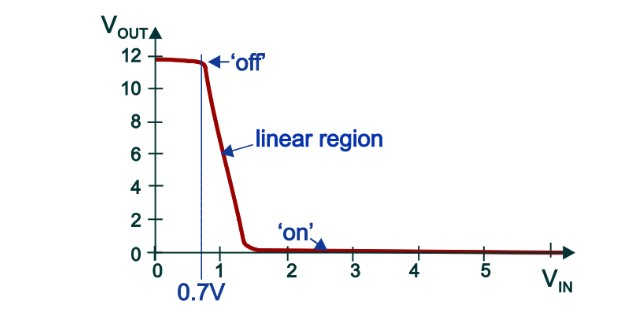
\includegraphics[width=0.45\textwidth]{bjt regions.jpg}\\
The transistor has three regions - cutoff (off); linear and saturation (on). 
\subsubsection{Cutoff Region}
$V_{in} < 0.7V$ The transistor is off. $I_C = $ $V_{CE} = V_S$. It is like an open circuit.
\subsubsection{Linear Region}
$V_{in}>0.7V$ Transistor switches on. It amplifies current as specified in the equation. As $I_C$ increases, voltage across the load increases therefore $V_{out}$ decreases.
\subsubsection{Saturation Region}
$V_{out}$ falls until 0. $I_C$ is at its maximum. Transistor is 'saturated' or 'fully on'.
\subsection{Transistors As A Switch}
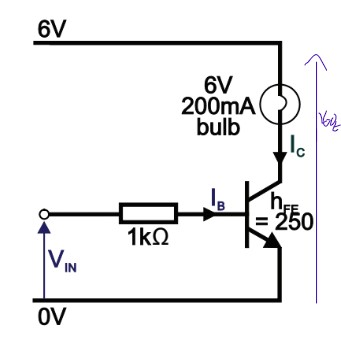
\includegraphics[width=0.3\textwidth]{bjt as switch.jpg}\\
This only uses cutoff and saturation regions. \\
When $V_{in}<0.7V$, the transistor is switched off. $V_{BE}=V_{in}$, $V_{out} = V_{s}$.\\
When $V_{in}>0.7V$, the transistor is saturated (switched on). $V_{BE}=0.7V$, $V_{out} = 0V$.\\
The base resistor (1K in this example) limits the current flowing into the base to prevent damage to the transistor. The lamp could be replaced by any load.
\subsection{Power Dissipated In A Transistor}
In the linear region, the transistor is on. $I_C$ is flowing but it has some voltage across it therefore power is dissipated. $\displaystyle P=I_{C}\times V_{CE}$

\section{Output Devices}
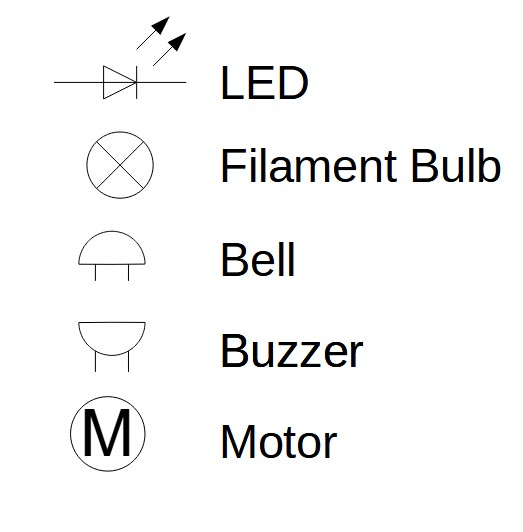
\includegraphics[width=0.45\textwidth]{outputs.jpg}

\section{Relays}
These are electromechanical devices. They allow us to control one circuit with another. They work by putting a current through an electro-magnet, this closes a switch on the second circuit.
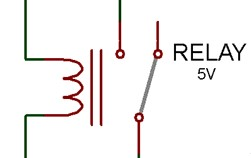
\includegraphics[width=0.3\textwidth]{relay.jpg}

\section{Back EMF}
Any device with a coil generates a magnetic field when turned on. When it is switched off, the coil collapses and generates a high voltage pulse in the opposite direction, this will fry components. We can add a protection diode to fix this.\\
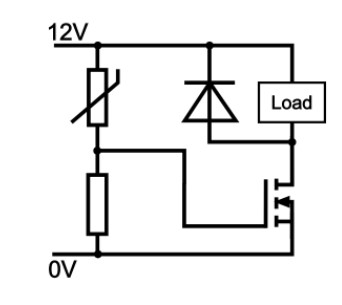
\includegraphics[width=0.4\textwidth]{backEMF.jpg}\\

\section{MOSFET}
Metal Oxide Semiconductor Field Effect Transistor.\\
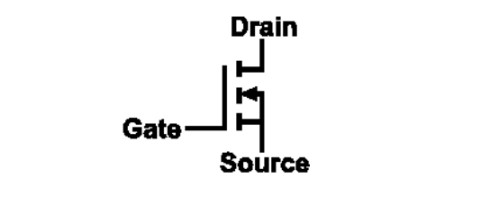
\includegraphics[width=0.4\textwidth]{mosfet.jpg}\\
The gate draws no current. The MOSFET is voltage controlled, the gate voltage controls the drain current therefore increased gate voltage means more current flows (because resistance decreases between source and drain). When $V_{in}=0V$, the MOSFET is off, no current is flowing. When $V_{in}$ reaches the threshold voltage (3V) current starts to flow from the drain to the source.\\
$\displaystyle I_D = g_m(V_{GS} - 3)$\\
Drain Current = Transconductance (Gate voltage - 3).
\subsection{Transconductance}
This is how much current increases for a given voltage increase. It is measured in $S$ (Siemans). Generally, it will be between 2 and 10 S. 
\subsection{Transfer Curves}
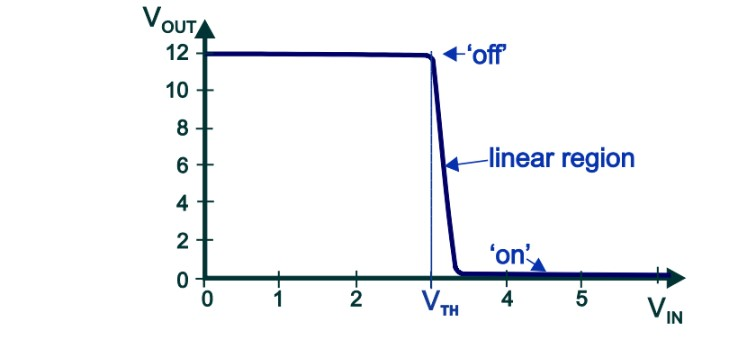
\includegraphics[width=0.4\textwidth]{mosfet transfer.jpg}
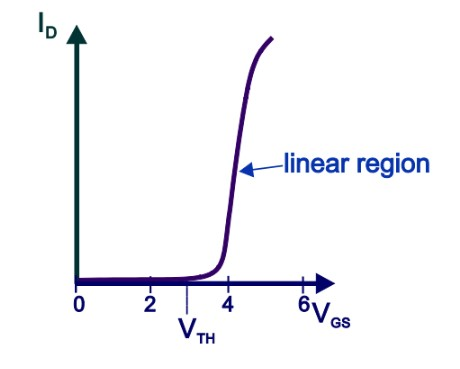
\includegraphics[width=0.3\textwidth]{mosfet iv.jpg}\\
The linear region is very small. MOSFETs make good switches. MOSFETs have very low 'on-resistance', $r_{DS_{ON}}\approx 0.5\ \mathrm{to}\ 1\Omega$
\subsection{Power Dissipated}
$\displaystyle P=I_D^2 \times r_{DS_{ON}}$
\subsection{Advantages of MOSFETs}
\begin{itemize}
    \item Low 'on-resistance' and high 'off-resistance' therefore good as a switch;
    \item Very high input resistance therefore draws no current therefore can be driven easily by logic gates/sensor subsystems. Unlike BJT, MOSFET will not load subsystem;
    \item Very high current handling.
\end{itemize}



\end{document}